% Created 2015-12-09 Wed 01:46
\documentclass[9pt,b5paper]{article}
\usepackage{graphicx}
\usepackage{xcolor}
\usepackage{xeCJK}
\setCJKmainfont{SimSun}
\usepackage{longtable}
\usepackage{float}
\usepackage{textcomp}
\usepackage{geometry}
\geometry{left=0cm,right=0cm,top=0cm,bottom=0cm}
\usepackage{multirow}
\usepackage{multicol}
\usepackage{listings}
\usepackage{algorithm}
\usepackage{algorithmic}
\usepackage{latexsym}
\usepackage{natbib}
\usepackage{fancyhdr}
\usepackage[xetex,colorlinks=true,CJKbookmarks=true,linkcolor=blue,urlcolor=blue,menucolor=blue]{hyperref}


\lstset{language=c++,numbers=left,numberstyle=\tiny,basicstyle=\ttfamily\small,tabsize=4,frame=none,escapeinside=``,extendedchars=false,keywordstyle=\color{blue!70},commentstyle=\color{red!55!green!55!blue!55!},rulesepcolor=\color{red!20!green!20!blue!20!}}
\author{deepwaterooo}
\date{\today}
\title{Life Love}
\hypersetup{
  pdfkeywords={},
  pdfsubject={},
  pdfcreator={Emacs 24.3.1 (Org mode 8.2.7c)}}
\begin{document}

\maketitle
\tableofcontents


\section{Original}
\label{sec-1}
\begin{itemize}
\item Created by Script Tutorials
\item License (if not mentioned otherwise in the files): \url{http://www.script-tutorials.com/terms-of-use/}
\item This readme is also a \textbf{three year review} for the three years that I spent to gain my Computer Science Master's degree.
\end{itemize}

\section{Residence Culture}
\label{sec-2}
\subsection{8/1/12-5/31/2013: 10 months lease}
\label{sec-2-1}
\begin{itemize}
\item My room-mate was originally came from Bangladesh for political reasons. And she has not even finished her local high school.
\item We took turns to do apartment cleaning.
\item Usually we got along well. But after she had complained me for quite a few times without logical reasons, I intend to ignore her in the apartment from about the second semester.
\end{itemize}

\subsection{8/1/13-5/31/2014: 10 months lease}
\label{sec-2-2}
\begin{itemize}
\item I rented the room to help a Chinese friend out, who was also a graduate student sharing the same major with me.
\item I asked the friend to find another girl to share the apartment.
\item This friend posted a print out page in SUB declaring that a Computer Science majored female graduate student from China was looking for a room-mate.
\item I called and blamed him that there was no reason for him to release identifiable information about me  publicly (It can almost clearly identify which was me from the university!) He admitted his mistake sincerely and I forgave him.
\item I rent the room partially because I just want to sign 10 months lease instead of one year. So in Jan/Feb 2014, when it's about time to extend new academic year, I found a Chinese friend to substitute me and continuing the lease.
\end{itemize}
\subsubsection{8/1/13-1/15/2014, first semester}
\label{sec-2-2-1}
\begin{itemize}
\item An American undergraduate boy rent the other room for the first semester.
\item He cooked less than me, and produced limited kitchen garbage. He put all kitchen garbage into my garbage can, and I was willing to take full responsibility for kitchen garbage dumping and cleaning.
\item I mentioned and was willing to take turns to clean bathroom, but he never do bathroom cleaning. Eventually I thought I may be too tough to force a teenager in his early 20s to clean bathroom, so I myself clean it all the times when I cannot tolerant it.
\item I paid \$55 wireless internet for half rent \$25 and first month (\$25 + \$5 bathroom curtain share he bought), and about \$25 for first month utility, and he continued to pay all the utility bills for himself and for  me as well (which means I didn't worry about bills for a few months).
\item When he wanted to move out, as I never tend to pick a room-mate at all, I agreed without hesitation.
\item When he moved out, he calculated the bills with me the last minute. I wrote a check to him to pay all utility for my part. But after he left, I realized that he calculated the wrong way (I should write \$25 less for utility), and he didn't pay back the internet \$25 rent.
\item I wrote email to him try to get my \$50 back, but he never paid even a cent back to me.
\end{itemize}
\subsubsection{1/16/14-5/31/2014, second semester}
\label{sec-2-2-2}
\begin{itemize}
\item The new room-mate was previous room-mate's friend.
\item I cooked once a week on Sunday evening for whole week. The new room-mate cooked more than I did, so we separated garbage cans in kitchen.
\item We did house cleaning in turns.
\item He set up online account to pay his half of utility bills online monthly, and I did the same for my 50\%.
\item He got used to watch movies/vedioes a lot without using headphones, so often he fall asleep with movies/music playing for hours during the evening. While during the spring semester I had my physical uncomfortable, and I had difficulty falling a sleep. I did get angry with him in late Feb about this. And I see doctor in early March for my illness.
\end{itemize}
\subsection{8/1/14-5/31/2015: 10 months lease}
\label{sec-2-3}
\begin{itemize}
\item During late July, early Auguest this year, it was very difficult to find cheap and appropriate room to rent.
\item At the time I had only two options. I wanted to share a 2-bedroom apartment with a Chinese girl, but the Chinese girl was instantly controlled by her advisor, and wasn't sure about her study plan for the year yet, she finally said she dare not rent the room for Auguest yet.
\item Then I had to rent this room from a university professor for 10 months.
\end{itemize}
\subsubsection{8/1/14-12/31/2015, first semester}
\label{sec-2-3-1}
\begin{itemize}
\item I have only one room-mate during the fall semester, who was a history majored undergraduate student and quit school, worked locally in grocery market.
\item The room-mate lives green and health, and always had tons of cans. I usually had only milk bottle and egg container for recycles, and she always had more than enough. I didn't know local recycle place yet, so I scheduled a few times with her so that we could go there together once, and since I had a car, I would be responsible to deal with recycling. But she always found excuses that she could not make the trip with me. And eventually I gave up.
\item The room-mate and any other person who rent the rooms from the same university Professor were not willing to work on the snow. I even cleaned the snow on the walking way on one side of the street for several times, tried to fit into neighbourhood culture. But nobody else worked on the snow, so I eventually gave up this item as well.
\item Whenever I made special food, I save a portion as a treat for her, but it feels she never liked it; And she never treated me anything.
\item We talk initially every once a while, but then she intended to ignore me in the house. Since I am a Computer Science major busy student as well. I was not hurt but rather took it naturally.
\item She forgot her key at home a couple of times, the first time I ride my bicycle home immediately and opened the door for her; the second time I had exam due, and called and invited her to come to close to my department (I studied in the department in most of the evenings), and gave her my key; I forgot the key at home a couple of times as well. Once I was near the house just realized the fact, and happened to see the other room-mate, and got opened by her. I remembered once I called her, she was working and not able to pick up the call, but she texted me. There was once I called and we talked in phone, and I went to her working place, picked up the key, got mine, and sent the key back to her at her working place (this went to her working place behavior happened once). 
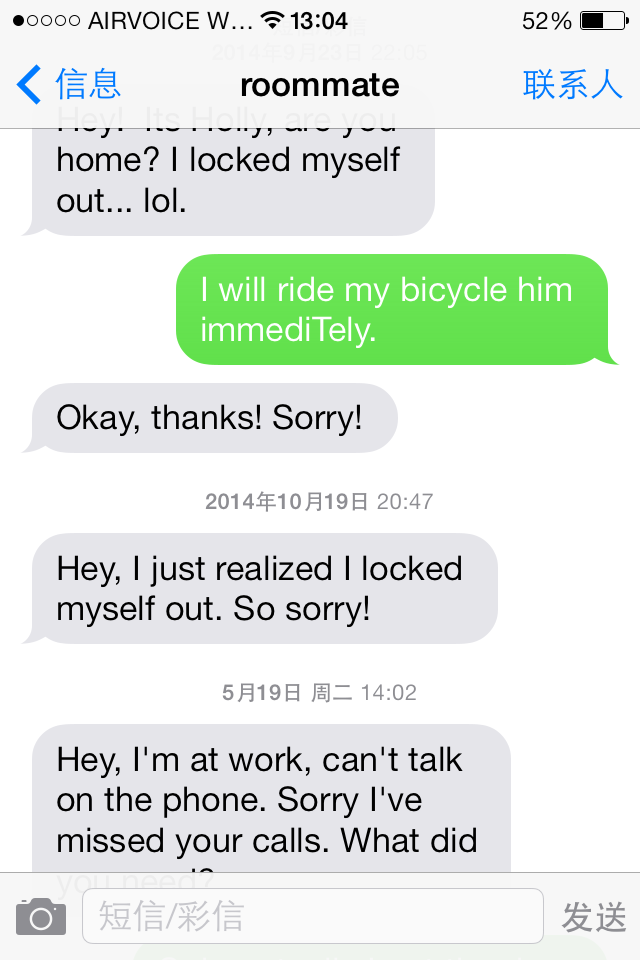
\includegraphics[width=.9\linewidth]{./pic/IMG_0427.PNG}
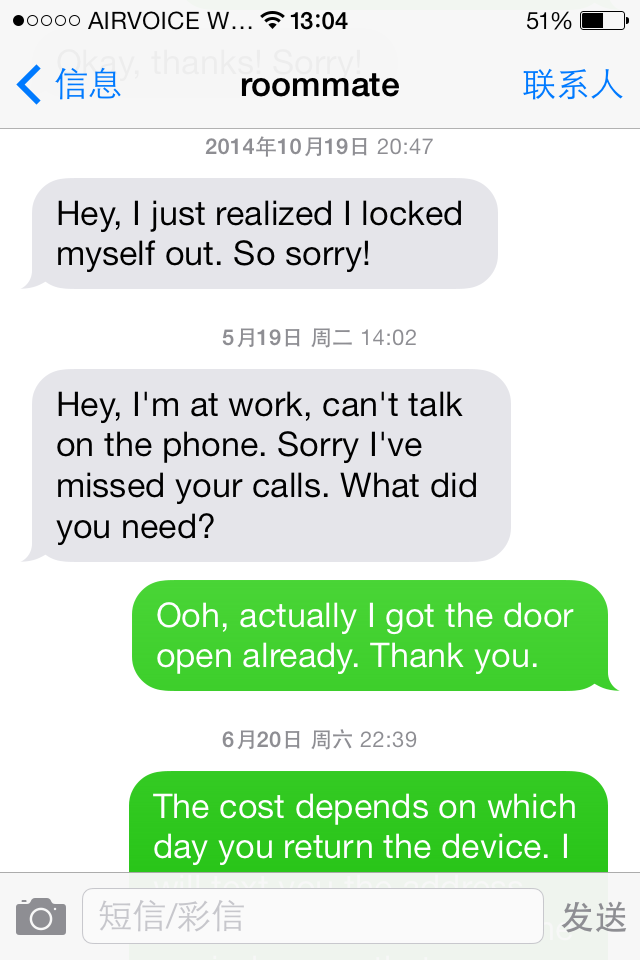
\includegraphics[width=.9\linewidth]{./pic/IMG_0428.PNG}

\item She was a midnight cat, and always do laundry in the late evenings, but I felt shamed to ask her do laundry during daytime, thought she may have plans during day time. So for the whole year, I tried my best to tolerant these kinds of behavior.
\end{itemize}

\subsubsection{1/1/15-5/31/2015, second semester}
\label{sec-2-3-2}
\begin{itemize}
\item The landlord introduced the new room-mate as she knew the student pretty well. I don't know why she wanted to live here for only five months, but I never asked.
\item Compared with the midnight cat room-mate who Usually did laundry up to 12:00am, the new roommie was a early bird, who waked up at about 5:45, and took shower every morning at around 6am. The washer and dryer was on the other side of one wall from my room, and the bathroom was on the other side of another wall from my room, while both room-mate's rooms were further away from these bathroom, laundry places and kitchen.
\item So for the spring semester, dryer run until 12:00am, and shower started at 6am. But still, these are just different person's scheduling, and I felt shamed to say anything, but rather try my best to tolerant these kinds of behavior even when I waked up every morning at around 6am, and after the shower, continued with kitchen noise.
\item The three different scheduling seems never run into each other. Or even when we were all at home, doesn't feel there was anybody talking to any other. But seems nobody cared about it neither.
\end{itemize}
\subsubsection{Conflicts with the first room-mate}
\label{sec-2-3-3}
\begin{itemize}
\item As the phone snapshot in ./pic/ folder showed, for the wireless internet device, on 4/17/2015 late afternoon, I have ride my bicycle all the way to local store check about closing my account and returning the device, and the man worked there asked me to bring back my device on 5/15/2015, because 5/17/2015 was Sunday and the store will be closed.
\item In that situation, I asked my room-mate to help return the device for me, and I paid her \$10 covering the 5/18/2015-5/25/2015 several days, during which days internet expenses should be divided by the room-mate and me. And the room-mate promised me she would do that for me.
\item The first time when she got back to me about this thing, her attitude was good, and was willing to be responsible for all the about \$53 cause the delay was completely caused by her.
\item But afterwards, her attitude was 180 degree changed, without any seduction from the university professors landlord, I cannot see any reason she would behave like what happened. 

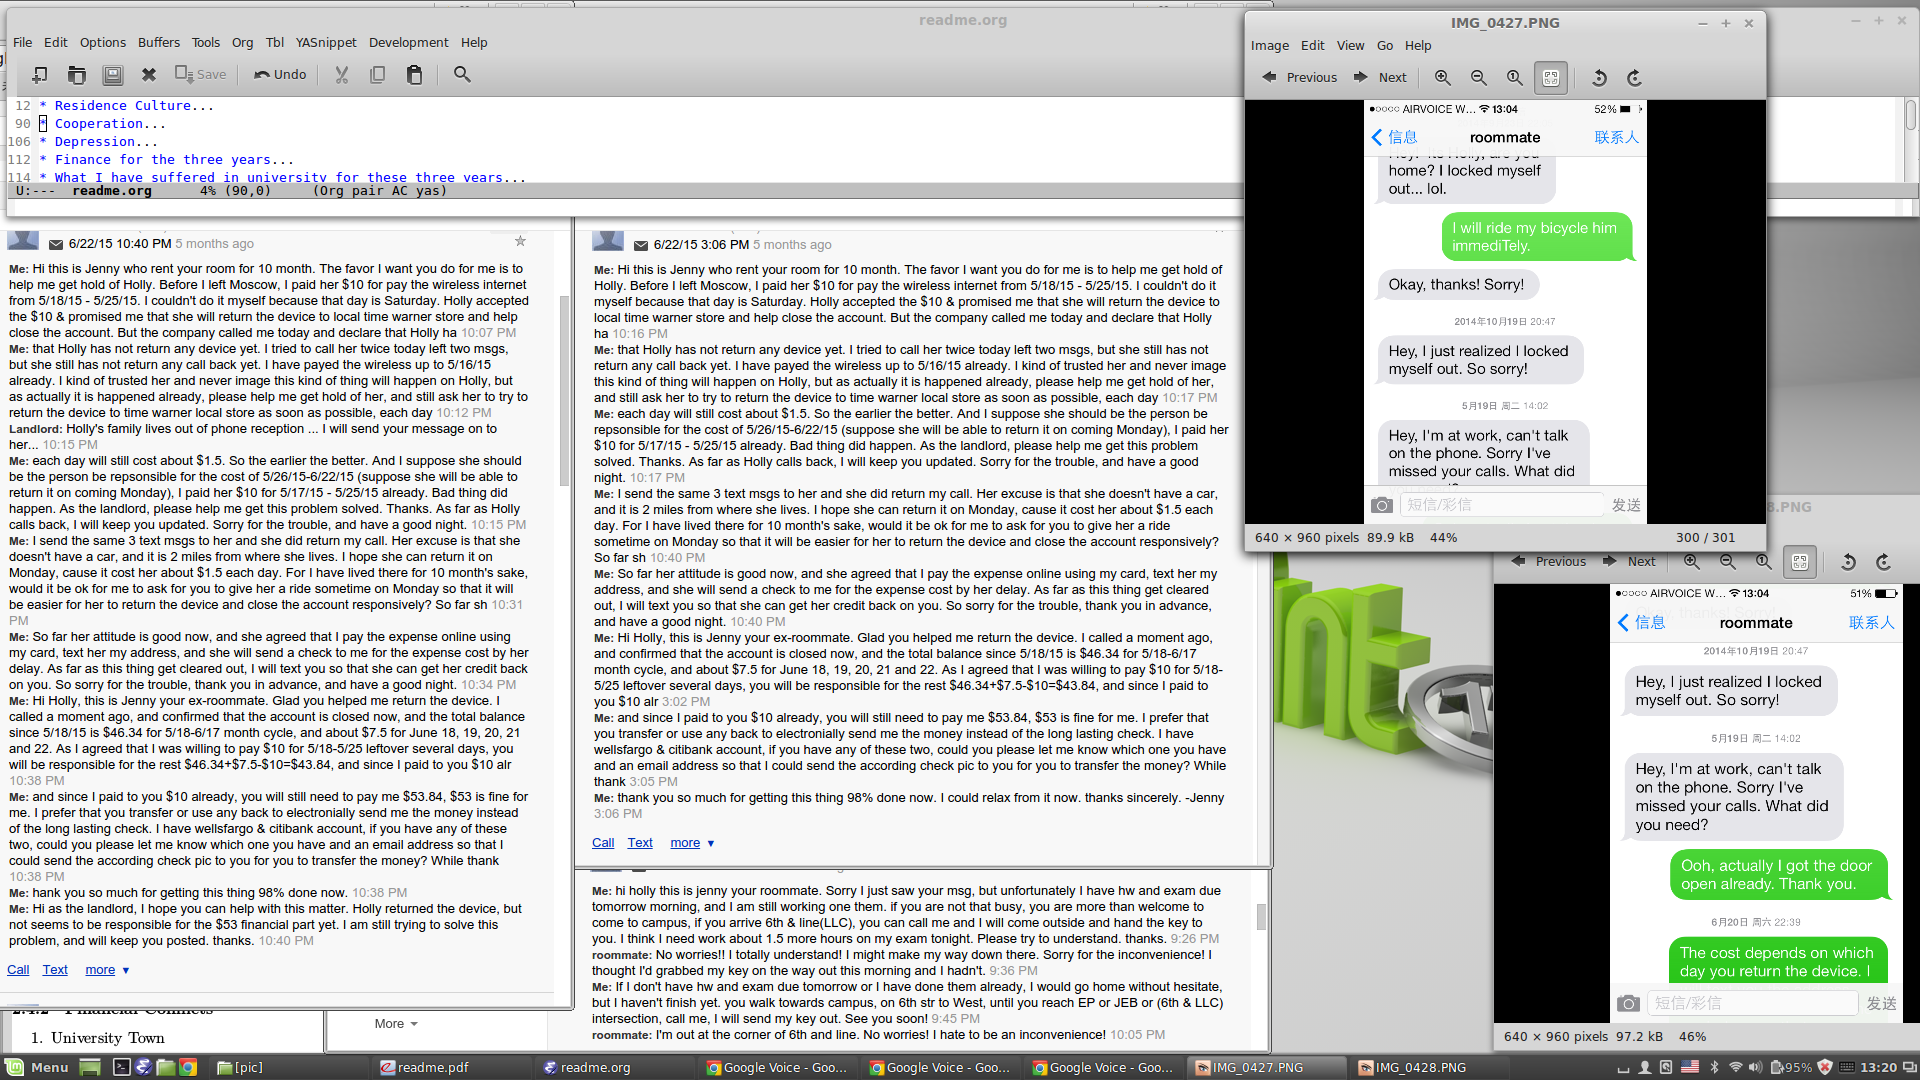
\includegraphics[width=.9\linewidth]{./pic/msgs.png}
\item From the communication msg we can cleanly see the landlord was lying about room-mate's not responding, which also serves as an on scene seduction trying to seduce her to behavior the way as the university professors landlord expected, and which I only realized after bad things happened.
\item I feel sorry that I lost patients waiting for room-mate's response after so many hours cause when I forgot my key, even at work, she had texted back before. I feel sorry that I thought she was not willing to be responsible for the bad things happened even I paid \$10 to her and she had promised to me that she would help me return the device.
\item When I got the first response back for the 2\% financial part from the policeman, normal human being can help understand how angry I was towards the so called room-mate, when this scene was set up carefully by the landlord and room-mate, I suddenly realized several facts that I had been kind and ignored before: 
\begin{itemize}
\item The room-mate's bad behavior of always doing laundry in the late evening was on propose;
\item The room-mate's bad behavior of always drying her close only after I finished taking shower (after my food court work) and was ready to study in the evenings in spring semester was on propose and she was meant to interfere my study;
\item The spring semester's new room-mate early bird wake up and took shower at 6:00am was a person found by the university professors landlord on propose, trying to reduce wake me up and reduce my study efficiency.
\item I had been a good room-mate never complained to them about their behaviors, while it seems I was too kind to be badly treated!
\end{itemize}
\end{itemize}

\subsection{Notes}
\label{sec-2-4}
\subsubsection{Residence Cooperation}
\label{sec-2-4-1}
\begin{enumerate}
\item California Residence Comparison
\label{sec-2-4-1-1}
\begin{itemize}
\item I spent 2.5 years in CA between 1/1/2010-7/31/2012. And I rent the same room in the same house from a Vietnam family in North San Jose for more than 2 years (27.5 months in total, 5/1/2010-3/15/2011, 6/1/2011-7/31/2012, 5/18/2013-8/31/2013). I don't have any conflicts with the family with three young kids/baby, and I even bought birthday gifts for the girls when it's their birthday, like music baloons etc.
\item In summer 2014 (6/1/2014-7/31/2014) I shared one bedroom with an international girl in down town San Jose and we got along well. I still appreciate the landlord's kindness that he didn't deposit my check until one month after I left, during which period which years, I was especially in financial problems.
\item During all the years when I lived/lives in CA (1/1/2010-7/31/2012, 5/18/2013-8/31/2013, 6/1/2014-7/31/2014, 5/25/2015-now 11/30/2015), I get along with all the landlord well, and I don't have any issues with any of them at all, in silicon valley CA.
\end{itemize}
\item My regrets
\label{sec-2-4-1-2}
\begin{itemize}
\item After the two years during when the room-mates were pretty much arranged by the university, I began to realize and miss the happiness and freedom of living with some girl with natural friendship. 
\begin{itemize}
\item I feel sorry that when I lived together with the Bangladesh girl I hadn't taken good care of her, especially when her life was slightly empty without husband around and with no study.
\item And during 1/18*/2015-5/14/2015, when I worked in campus food court and I have chance to work together with the girl and her husband, I tried my best to cheer her up and took good care of her when she and I were in the same shift also because she was pregnant and were not able to work on heavy things. I believe she could feel the kindness that I treat her.
\end{itemize}
\end{itemize}
\end{enumerate}
\subsubsection{Financial Conflicts}
\label{sec-2-4-2}
\begin{enumerate}
\item University Town
\label{sec-2-4-2-1}
\begin{itemize}
\item The room-mate from 8/1/13-1/15/2014 owned me \$50, but he never returned it back to me, which was mentioned in \url{https://github.com/deepwaterooo/MyAutobiography/blob/master/part3_deepwaterooo-Autobiography.pdf} part3 chapter 16, page 157-163. On Page 163, I wrote to him trying to get my money back, but I never received any response from him.
\item The history-majored female room-mate from 8/1/14-5/31/2015 owned me \$32 as she declared she wanted to be responsible for, but I never received the money order she mailed. And towards jerks who was seduced by university professors and reported me to police department without leaving me any feedback, I would never want to cooperate with her ever again.
\item All the financial cases happened on me were happened in university town, together with what have happened during the past three years, I have confidence and clearly believe that it were the American university Students' bad behavior, and I should not be responsible for theirs means at all.
\end{itemize}
\item CA: During all the years when I lived/lives in CA (1/1/2010-7/31/2012, 5/18/2013-8/31/2013, 6/1/2014-7/31/2014, 5/25/2015-now 11/30/2015), I get along with all the landlords well, and I don't have any issues, financially or whatever, with any of them at all, in silicon valley CA.
\label{sec-2-4-2-2}
\begin{itemize}
\item I love life and love living (which was the reason I failed to kill myself when I was 19.), and I fit into Industry company culture well as well. 
\begin{itemize}
\item In all the companies that I worked, I treat my coworkers well. If somebody treats me nice, I do at least the same back, treats back for lunch for lunch sharing etc.
\item In Nielsen Online, once the site had baby-shower for two new-borns, each of us were suggested to pay \$15 for preparing gifts for the two, I paid mine without hesitate; while the middle-aged Chinese female in the team didn't.
\item In December 2010, I donated \$1000 back to the university Statistics department cause I was working then, and I was financially slightly better those years.
\item All the slanders, set-up scenes were cleared out. I highly suspect all the slanders were produced by some website trying to make money, just like some university would want to seduce students set up scenes to destroy its own international student's reputation by all means.
\end{itemize}
\end{itemize}
\end{enumerate}

\subsubsection{Conclusion}
\label{sec-2-4-3}
\begin{itemize}
\item I guess it was just a few American University Undergraduates individual student or quit out who are irresponsible and have problems, not me.
\item I don't have any cooperation problem in residence environment, or in industry company working environment.
\item I don't have any kind of selfish financial towards room-mates or coworkers.
\item The slanders trying to build a nasty figure who produced them, reflected whose low-profile personality, or institutes reputation, instead of destroying mine.
\end{itemize}

\section{Cooperation}
\label{sec-3}
\subsection{Course Projects}
\label{sec-3-1}
\begin{itemize}
\item I barely had any team course project experience, only 3 times:
\begin{itemize}
\item Spring 2013, as a second semester CS majored master student teamed with a Math Ph.D female with no programming experience, though the project didn't process successfully, I met course instructor weekly and developped all the codes needed until the course instructor were satisfied with the performance.
\item Spring 2014 (or fall 2014/2013 ?), the team Project for ZigBee wireless communication for one of my adviser's course, I cooperated well with other 3 to 4 team members. There was no conflicts at all.
\item Fall 2014 Senior Design team project was completely a set-up trap against me. All other teammates got promoted by their behavior from the university.
\end{itemize}
\end{itemize}
\subsection{Industry Working Cooperation}
\label{sec-3-2}
\subsubsection{Nielsen Online}
\label{sec-3-2-1}
\begin{itemize}
\item I have worked here twice up to 14 months (5/10/2010-2/17/2011 \& 8/10/2011-1/6/2012);
\item The team configuration is: 1 project manager, 1 Chinese group leader guiding another middle-aged Chinese female and me, and 2 to 3 Indian females. As a fresh graduate contract, up to 14 months, I never have any conflicts against any team members or coworkers. And I fit the company cultural pretty good as well, which was covered in 2.4.2 Financial Conflicts 2. CA part already.
\end{itemize}
\subsubsection{Samsung Semiconductor}
\label{sec-3-2-2}
\begin{itemize}
\item Worked here as a summer intern for 2.5 months (6/17/2013-8/30/2013).
\item Guided by a senior mentor for 1.5 months, and by a young while much experienced mentor from cutting-edge technological project experiences and programming side for about 1 month.
\item Guided by a great mentor, I got great practice and experience, and I admired the mentor so much that I could think positively naturally. For example, my last project was only reviewed once on the last day after 11:00am. And we had team group lunch for farewell up to after 1:30pm, almost 2pm, which left me less than 3 hours in the afternoon and I still had to fix a UI bug which I didn't have any idea yet. I drunk several cups of coffee, thought aloud, made all my effort to make the project done and work without wasting any time recall if the criteria was specified before, and/or if so, when? That was the most encouraging and positive experience I even had during the past three years.
\item There was no conflicts, rather than developping better subteams, getting project tasks well done, promoting problem solving efficiency, as well as creating better learning and practice environment for ungraduated interns, which in my opinion, is a great company culture that silicon valley high tech should follow, and I appreciate this culture a lot!
\end{itemize}

\section{Depression}
\label{sec-4}
\begin{itemize}
\item I came here in US on 8/10/2006, and I went to CA in May 2008. How many times I got depressed in University, as many times I got cured by visiting and staying in CA.
\item Silicon valley is my hometown in US, instead of the university, where I got severely depressed in Spring 2015. 有人说,这个春天我究意怎么了?是的,学习上工作上交友上我一向都还乐观自信热情大方,但自去年秋天senior design项目意识到学校系里设的陷阱后,我被没收了学生办公室,整个校园严冬凛冽刺骨的寒风般氛围就像敌人举着明晃晃的钢刀向我杀过来。。。这个春天对我来说实在太痛苦,在食堂打工,清楚地知道食堂里所有manager都在想方设法地by all means抵诽诽谤我,阻止实习公司给我工作机会,并试图毁掉我所以可能在工业界工作的机会,逼我读博士,可我,除了小心翼翼又能怎样,长期以来被学校的孤立/以及食堂里时时刻刻感觉着的各种诽谤,让我的这个春天极其煎熬,神经极度敏感,整个人处于压抑状态,几乎成了神经病。四月后看清周围的形势,知道网上究竟是哪方倒乱,才稍微有种船到桥头自然直的些许放松。只有后来到了加州后,才能感觉自己的状态在从痛苦中回塑。这校的校园,愿我永远不要再踏入一步!
\end{itemize}

\section{What I have suffered in university for these three years}
\label{sec-5}
\subsection{footprint \& global agreement}
\label{sec-5-1}
This part has been posted on part4 chapter 29, post it here as well for convenience. 

(me\textasciitilde{}) ((me\textasciitilde{})@xxxx.uxxxx.edu)

Sent:        Tuesday, November 18, 2014 6:42 PM
To:        
e [e@xxxx.uxxxx.edu]; 系里小秘 (系里小秘@uxxxx.edu); 代课老师 (代课老师@uxxxx.edu); Alves-Foss, James (jimaf@uxxxx.edu)
Cc:        
m [m@xxxx.uxxxx.edu]; p [p@xxxx.uxxxx.edu]; r [r@xxxx.uxxxx.edu]

Hello e, and the related department, 这部分不要

As I pointed out that it was all your fault which leaded to these whole confusion, and have stated in the meeting on Saturday that, I was going to write a email as a footprint to prevent you from future suffering, and help myself clear my life here in U of I. 

Facts:

\begin{itemize}
\item On team meeting \textbf{10/7/2014, Tuesday}, always being active and fast towards projects, m suggested us to install Qt Creator, downloaded Qt Creator sample codes into GitHub. He helped p installed the software on Windows, and I did mine in Linux. m's sample code created and menu bar "File" command already, and "Exit" from submenu of "File".
\item On team meeting \textbf{10/7/2014}, the same Tuesday meeting, you excused yourself having trouble with MS c++ IDE, and would do rather the IDE package than the independent Qt Creator, and r spontaneously offered helped to you that he was going to help you look into MS c++ IDE if you needs any help.

\item On team meeting \textbf{10/7/2014}, the same Tuesday meeting, m, p and me got our Qt environment ready, while r and you chatted and talked about your compilers, and draw the "Design Flowchart" on whiteboard and listed, "C\# prototypes organized uml diagrams, prototypes/language training Diagrams", and assigned to r dated "by coming Tuesday r", deadline 10/21/2014; "Design/Docs/Exact Class Diagrams" deadline 11/11/2014;

\item On team meeting \textbf{10/7/2014}, the same Tuesday meeting. In the end of the meeting, as you were the respected one with full communications with course instructors, and could draw exact deadlines like listed above, when asked about tasks before next meeting for Qt Creator coding training part, you clearly stated as far as we could create one button and exit from there, we are good. m insisted that "I already did that", but you blocked the whole team from processing by giving no followed up tasks/assignments on Qt Creator.

\item On Team meeting \textbf{10/9/2014}, the meeting with instructor Professor 代课老师, you covered part of the project agenda; and you \textbf{begged*/kind of *forced} r to stand into front and speak of something. And r did follow your call and covered parts of the c\# codes on color Pale, color wheel, Grid, Main form. I specifically asked if r could draw a clear class diagram for C\# design, he looked into Professor 代课老师, and the professor gave enough tolerance to r that we didn't necessarily need any class diagrams even you listed it on whiteboard two days ago.

\item On \textbf{Friday 10/10/2014}, in CSAC between 4:00-5:00pm, I asked if you have base version tower light interface, you said no, and we agreed I sent email to ask help from team members; The same evening I sent two emails out, even call for gathering and preparing for coming Tuesday's snapshot day, as the team manager, you completely ignored my email and leave me no chance to prepare for snapshot day by having asked p only (without letting other team member knew about it) to work with you to prepare the snapshot day. And what a probability that our team was completely forgotten by the course instructor as well, not shown at all in the email list the instructors sent out.

\item On week \textbf{10/12/2014-10/18/2014}, because all of you have compilers, we didn't meet. 

\begin{itemize}
\item On Team meeting \textbf{10/23/2014, Thursday}, after having checked with Professor 代课老师, you listed us on board in m's office, that we have assignments need to be done, including state diagram, wiki page, class diagrams, GUI design and description. And e you wanted to work on Wiki page, m would work on state diagram, I wanted to work on GUI design, r and you would work on class diagram, and p jointed me to work on GUI. You set very high standards on GUI doc name conventions and even suggested that we need to consult some other department, but my sub-team member p argued it back that we don't need to.

\item On Team meeting \textbf{10/23/2014, Thursday}, In the same meeting when I picked this GUI design assignment, as an always considerable teammate m is, he argued me, "do you understand what a GUI design is? -- To create a clickable interface that we as a whole team could link functionalities on the buttons later on.  As far as I understood, I knew clearly what I was supposed to do, as clear as any other team member knew. And nobody ever rejected any of m's reminder opinion on the GUI or mine on this GUI design at all.
\end{itemize}

\item On Team meeting \textbf{10/28/2014, Tuesday}, I didn't really remember when m checked in and uploaded his state diagram onto Google drive, but it should be sometime during this week. We chatted and discussed about some details about merging two paths/pattern. r did draw some pic on the board. In the end, you asked r to send this photo pic to you, and asked from r about the same, but I never received any pic from r yet about that meeting's draw on board. 

\begin{itemize}
\item On Team meeting \textbf{10/30/2014, Thursday}, by this time, m probably has checked in his state diagram already, and we emphasized on e, you work on wiki page by coming Tuesday; and r and e work on class diagram, and p and I work on GUI and GUI docs. As m has checked in already, and been emphasized and deadline was coming, I set my mind to work on it.

\item On \textbf{Friday 10/31/2014}, on the mornings somewhere, my sub-team mate p taught me how to create form-based Qt Creator interface. I had fun building some buttons. And between 11:30-1:00pm when you showed up in CSAC, I was working on the GUI, and I showed my currently working GUI form-based interface to you. You seemed to feel exact but good or bad, you didn't say anything about it.
\end{itemize}

\item On \textbf{11/4/2014, Tuesday}, for the first time, you skipped me from the team meeting with no excuse at all. This wasn't the first time that we skip a meeting. When it was you guys' compiler exam week, we skipped team meeting once. And This was the first time you all moved downstairs to have team meeting in m's office instead of in CSAC on Tuesdays, and as the team manager, you leaded the team without notify me about the team meeting. And your coldness in your email freeze my mind, it was like finger pointing and clearly saying that me, as the only one who ever missed the meeting, was the one who didn't do anything at all as you descried p to me the followed day. And I was so considerate and tolerate to you by just saying that "your email surprised me a little bit".

\item On \textbf{11/5/2014, Wednesday}, you didn't reply to my Tuesday evening's email and chose to step by our office, and chatted to me for several minutes. During those several minutes, the points you made includes:
\item Checked me if my sub-team mate p was doing anything at all. Almost as motivated as I am, as everybody knew p has at least prepared the snapshot day's image design already, so did I, I explicitly emphasized that to me, p didn't have such a problem at all, and I always has my full confident on him.
\item When you insisted that later on you will send email to remind us about meetings, I wanted to make it clear that you didn't necessarily need to send us email at all, but you made a point that r is a person prefer oral works, and doesn't like any reading and writing at all. Yet still you insisted you would send email out so that you could remind r because you need to anyway.
\item Combined your coldness on 11/4 email and the scene you prepared for me, if later on I wouldn't be able to produce the clickable GUI, I would be basted to death. Could the scene/environment be any colder on me? Why do I need to suffer this?

\item On \textbf{11/6/2014, Thursday}, on the mornings I received 代课老师's email and he clearly stated that he will have access to our emails. And I agreed I have no problem with that at all with all my reasonable guess what happened during the mornings.

\item On \textbf{11/6/2014, Thursday}, since coming Tuesday will be the design review day already, and nobody ever brought up the design review thing ever, nobody! We were mainly on the r's performance thing, and you asked r to try to mimic the presentation in m's office without any writing material. And r clearly asked if we could have our GUI interface ready that would be something great. I also wished that I could finish have my interface so that we would be able to demo it, which according to me, would greatly improve our grades as well. As that time, e, you tried to be a considerate manager without giving me any pressure by, simply completely ignore the fact that I have been working on it, and have at least showed it you once, simply clearly stating that if r really think we should have something to demo, e you as the team manager, would simply ask p to create a short video to demo the functionalities, which was what happened during the coming weekend.

\item On \textbf{11/6/2014, Thursday}, after our team meeting, which ended at around 4:30pm, my sub-team mate p and I went to CSAC and I asked him about the difficulties that I have, like how to add an image using form-based interface. Together with me, p and I used two laptops searched for some time. As frustrated as I was, p called you discussed about the difficulties that we encountered, and as the team manager, still you didn't say anything about the clickable GUI design related issues, rather than relax us by stating that we could still simply create an image based interface just like what p did already for our snapshot day, as far as it's slightly better, like we agreed that our moving direction should have 8 directions instead of 4. It was 5:00 already, I felt I contributed to the team too limited, and p and I agreed that I would work on the image and docs during the weekend, and our sub-team would meet on Monday at 2:30pm to clear work out. It was during weekend when I really worked hard on the GUI, in the email I moved the GUI docs works to p so that in sub-team he would be able to contribute as well.

\item Before Tuesday's meeting, you have your excuses like you have TA lab section on Tuesday mornings, but you never took your imitative to offer a time like sometime on Monday or weekend to review the slides of r's presentation or offer any guide.

\item On \textbf{11/11/2014, Tuesday}, Design Review with CS related teams gathered together. Before class, I noticed that e you were asking classmates if they have met any person who didn't know the correct way to communicate in a business manner. And during the day's 5 team presentation, Professor 代课老师 gave r too long time on our review with r spent half of the time description on feature that I didn't finish on the time Editor. I did feel bad about you guys by behaving like this. Professor 代课老师, you and I talked after that days' design review class in the same classroom, but I got sick of the environment already. Professor 代课老师 said that he didn't read all the emails, I wondered if he "did", could the situation be any better? And at around 4:30, I received email from human resources, whatever the contents are in the email, I felt pressed.

\item The followed several days communications were completely a mess, and personally I don't even want to recall all these things.

\item On \textbf{11/13/2014, Thursday}, you casted a great anger toward the whole team by blaming us that we missed the point of design review, which I have pointed it out on last Sunday's email already but you paid no attention to it, let alone correct us at all. But as far as you recognized in the end of the meeting, you blamed yourself you didn't know what the fxxxxxx you were talking about in the end before leaving the room, I tolerant your anger, forgiven you and didn't make any sound.

\item On \textbf{11/15/2014, Saturday}, you applied your advantages by taking team meeting notes. You didn't offer any suggestions except that you explicitly specifically blamed that it was my fault misunderstood you. At this point, I cannot tolerant you anymore, and stated to you clearly that it was all your fault by misleading the whole team do wrong things at the wrong time, and I would write to you make this clear to prevent you from repeating such situations. I must be too anger to blame it was you, but actually it could be the department as well, cause you have been the only person keep close relationship with the department, and you were entitled absolute admire by an undergraduate TA.
\end{itemize}

e, please understand that I never take any initiative to hurt any other person. Whenever I need to stand out to say something, I stand out only when I got very hurt and cannot bear the situation any more. It was you, who was extremely unreasonable, that forced me to stand out, clear everything clean, so that later on I won't suffer any more from these afterwards. You were the source produced all these troubles. 


First of all, I appreciate the TA I got for this fall semester. But please all help to realize the facts that I listed. About the TA: as clear as i demonstrated, I appreciate if I could get it, but I won't be any aggressive to fight for it at all. Maybe I am writing trying to reach global agreement between the department and me. 

\begin{enumerate}
\item Early on 10/23/2014, cs120 lab8 section 6, I covered email and demoed emacs presentation slides generation using org-mode, just wanted them get encouraged and learn the command-based editor. When I realize the afterwards influence, with my current advisor fully supported me to demo by design the lab8 to be one easy function only, the coming Tuesday 10/28 (the emacs slides were still left there, but I didn't cover that much and didn't demo org-mode slides generation any more at all), I hide my shining avoid any emacs demo just asked the section 4 to add one line of global-line-number configuration for their convenience. I just wanted to keep low-profile life.
\item After the unfortunate Emacs thing, Dr. Soule fully supported Josh, the other TA's idea about curses window for assignments. For me, it was just a wrapper class like any other project that I can do. I have my priorities for works to do, I didn't pay enough attention to that, but it was followed by e's aggressiveness by picking my accent. I am perfectly ok with my accent.
\item Dr. Soule fully supported towards e and Josh, and the assignments extended one week, the students looked down on me, and I have even received "patent" emails during those days. How the environment could possibly appeared to be that way? I was driven sad by the environment and studies a little bit on <curses.h> library, and demoed the class on Thursday's lab to protect myself from any further suffering. But still, it was just a wrapper of a source library, patent?
\item Compared with a TA for spring semester, I would rather prioritize my time so that I could make good preparation for my job searching, and get graduated smoothly from this department. And that's the reason from very beginning from emacs demo week, unlike e as aggressive as she behaves; I have been completely outside this TA aggressive war. I will get graduated.
\end{enumerate}


I got pretty much all Bs from my previous courses, like cs210 programming languages, cs570 AI, EC, which ones that I liked too much, though I did feel very unfair about some of them, like cs210. I wrote a 500 line of Elisp code to make one tic-tac-toe move within my first month here in U of xxxx. But still with limited homework scores, I got B still. With all these grades, I must be very stupid to progress well at all. And on 11/17/2014, fault tolerance, Dr. 代课老师 was saying some minds don't seem to turn around at all. According to all the facts happened during the pass more than two years, it must be especially stupid me that was not able to study well, nothing to do with the instructors, nothing to do with this university at all\textasciitilde{}

I have been brave to solve my technical problems, but now when I looked back to review this process working with you, and what has happened during the past two years, especially during this year, I felt frightened. I am a girl grown up from the countryside in a developing country with all the suffering during my childhood. I had all my out-of-state tuition fees waved for my Statistics master's degree. How could I ever imagine that I was going to suffer all these discrimination on me, good or bad, all Bs for my courses, separation from the rest majority of classmates and so on? Tortured by personalities like yours, I always suffered from feeling unsafe, and this unsafe feeling dragged my life miserable. If I know any of this detailed information, if we could rewind the time back, I would never want to step into this department ever again! And in the future, if I have any choice, I would not want to come back to this department environment again! 

Up to this point, I wonder how many professors in our department now are still dreaming that I would continue with a Ph.D in this department. We have two Chinese Ph.Ds, Xin and Jia, both of whom chose to stay here for Ph.D without even trying to work in industry by applying OPT. It's their personal choices to stay in UI for Ph.D without OPT after masters, but as clear at this point as we shall all reach and agree, it will never happen on me! I AM GRADUATING in Aug 2015\textasciitilde{}! No regret, no come back. 

I learned that all the instructors, Professor 代课老师, who is the only master's degree instructors here in our department; Dr. Soule, who doesn't necessarily qualify for a Assisted Professor here in UI before, was all completely brought up to be an associate armed with best students during the tenure tracking process, which is similarly happening on another assist professor right now as well . Since all those persons who gave me hard time (Dr. Soule blocked me from having an industry offer which company I have worked for earlier in spring semester by covering cooperative convolution in his EC class during critical decision time) are all appreciate to Dr. Alves-Foss, now I do begin to think if it is the truth that actually it has been Dr. Alves-Foss who designed and directed the whole process of blocking me here in U of xxxx. And also he will be "on war" for coming spring semester for cs210, I will stay tuned, sharp my eyes and ears to see what's Dr. Alves-Foss's opinion on this thing. Will he work hard to block me from graduation, from finding a job, or he may even help me find a job, or could simple just let me go? I look forward to see his response towards this whole thing. 

-- (me\textasciitilde{})

\subsection{Quick Summary}
\label{sec-5-2}
\begin{itemize}
\item I didn't want to continue with any MS computer science from this university when I appeared on campus early Aug 2012, and learned from the department that I should only register 7 credits for my first semester. It were the famous Professor from the department and mh previous advisor tried their best to leave me there by allowing me to register more courses, at least for the first semester at that time. And at that time, their attitude was good sincere and admirable.
\item The department tried to block me from choosing Statistics related courses on one side, and tried to block me from processing and developing well from Computer science major as well, not by forbidden me to choose those courses, but rather by giving up offering those courses on propose for my later semesters. I had successfully wrote a tic-tac-toe 500 lines of lisp code as a homework. I am confident about my course work, and I know I have great skills rather than the transcripts represented.
\item I have spent 3 years for this MS Computer Science degree, what were the skills and ability I had by 8/7/2015 was a full reflection of the university/department/Computer science program teaching performance.
\item They tried their best to seduce me to continue with a Ph.D while forced me turn in student office and get rid of my efficient study environment with no reasons, as well as produces chaos living environment for me on propose.
\item Even I ranked high on student performance, they gave me B by using all kinds of tricky means. And they didn't allow me to select any more courses in Spring 2015 by not offering any TA. This leaves me no chance to take any other courses that I was interested. They didn't give me any opportunity to improve and enhance my technical skills.
\item Since the very first semester, the grades I got was not fair for me at all. And any classmate who had any kind of admire on me got punished by the department on propose, which results in during the three years, no students dare to get close to me. It was such a lonely program and department without any warmness. I have been the most lonely student from this department for three years. Gosh, I can barely recall these details. It is painful.
\item There were twice the intern company was trying to offer me working opportunities, while twice, the university blocked me from getting it.
\item In this university, humanity is such a joke that international students need carefully consider if they want to take a try.
\item As I mentioned before, after recalling what had happened on me for the three years, I feel shamed that I had ever donated \$1000 for such a university.
\item I have seen doctor and made ultrasound test about my physical disease in March 2014, and after all these years progress since surgery on 7/29/2001, I highly suspect that I could very possibly have difficulties to get pregnant and have my own baby.
\item The local police department cooperated with the local court asked my cousin set-up a permanent court order up to 3/21/2017, and I have to wait until that day.
\item The unreasonable thing was that I was not given that piece of information until 2/27/2015, and the permanent order was set up on 3/21/2013, which means they wasted my life for almost 2 years! Could anybody give me any reason I should NOT know this information? This is also human beings and local police department and local court.
\item What I need is just a computer science related job to make a living. I don't know why the university was so anti-sociel and leaves me no way to survive!
\item One day when I wasn't able to insist my love, I know it was this university and local government and local court that destroyed our lives. \textbf{Only the university without any humility nor even fair always wanted to separate the lovers apart to escape 社会和舆论的谴责 for their bad behaviors they have done on me during the past three years。 But is there even at least one party who wants to separate when they are in love for more than FIVE years already (ever since December 2010)? If I have a job, how could I want to lose mine, especially when it's always so difficult to meet the one?}

\item One day when I realize that I seriously won't be able to have any kid, and it is because these years of delay, I promised I will hate the famous Professor from this department and my previous advisor, together with the whole computer Science department to death!
\end{itemize}

\section{What am I going to do with my life?}
\label{sec-6}
\begin{itemize}
\item What am I doing with my life? What am I doing with my life now is the full reason I am writing here to spread all my stories and all the suffering I had here from the university worldwide. So that international students could have more information and better understanding about the international students' campus/off-campus lives and how they are controlled by the university.
\item What am I going to do with my life? Should I take any further risk to try to continue with any Ph.D after having suffered all of these for three years? go to hell\textasciitilde{}!
\end{itemize}

\section{Finance for the three years}
\label{sec-7}
\begin{itemize}
\item I have \$27,000 savings before I went back to the university.
\item The major uses of the savings are listed as followed:
\end{itemize}
\begin{center}
\begin{tabular}{lrl}
\hline
Items & Amount (\$) & Notes\\
\hline
Tuition Fall 2012 & 10500 & \\
Tuition Spring 2013 & 10500 & \\
Health Insurance & 1392 & one year, 116/month, for female, includes pregnant cov as required.\\
Rent Room & 2500 & 10 months\\
A used 98 Buick car & 1200 & with 219000 miles on wheel when I bought\\
Rent Room for Summer in CA & 1500 & for 3.5 months\\
gas back and force CA & 250 & once during summer\\
pay to local court & 50 & \\
\hline
Intern for Samsung Semiconductor & +10000 & after tax, for 11 full week, \$36/hour\\
\hline
Tuition Fall 2013 & 10500 & \\
Health Insurance & 1392 & one year, female, includes pregnant cov.\\
Rent Room & 2920 & 10 months\\
IAA Collection for Ambulance & (832.20+416.10) & 832.20 for ambulance, and 416.10 for 50\% collection fees though I never received their letter\\
Tuition Spring 2014 & 200 & waves out-of-state, TA \$4000-\$200 wasn't able to cover even in-state tuition, let alone living\\
tax return & +3500 & \\
fixed the car & (250+250) & 250 for gas pump part ordered from local auto zone, and 250 for labor paid to auto shop\\
Rent Room for Summer in CA & 700 & for 2 months, share one bedroom with a girl\\
gas back and force CA & 250 & once during summer\\
\hline
Tuition Fall 2014 & waved, +7500-4000 & TA offered \$7500 before tax, \$4000 was spent for Fall semester in state tuition fees\\
Health Insurance & 1400 & one year, female, includes pregnant cov.\\
pay to local court & 150 & \\
Rent Room & 3000 & 10 months\\
Bob's food court & +3500 & \$8.35/hour, about 20 hours per week labor in campus food court,\\
Pay to credit cards & (135+60) & paid about \$135/month to citi credit card, loan rate APR 20.99\%, and \$60/month to wellsfargo\\
\hline
\end{tabular}
\end{center}
\begin{itemize}
\item My citicard limit is \$5000, and wellsfargo is \$2500. For the past two years, I just struggled all the way to pay the \$200 each month debt.
\item The program asked me to pay full tuition fees each semester for the first THREE semesters.
\item The forth semester TA \$4000-\$200 was not able to even cover my in-state tuition fees, and I had to spend on credit card all the times to make a living.
\item The fifth semester was offered \$7500 before tax, but up to then, I had to pay \$200 each month to credit cards already.
\item the sixth semester, when I had been fully armed to learn more efficiently, the university/program leaves me no opportunity to learn at all.
\item The university/program said that the first three semesters they never gave me TA because I was not qualified, and the sixth semester when I was qualified the famous professor said I got 30 credits already (30 credits makes a MS Computer Science without a Bachelor's degree, that's University of XXXX), and I should graduate. Study environment factors includes: 
\begin{itemize}
\item Got my student seat office key back on Nov 21, 2014 on propose, because they thought I was too efficient studying using a graduate student office seat, and un-blockable.
\item By controlling living environment, the history majored student did her laundry only on evenings when I was studying, up to 12:00am.
\item By offering NO TA for me for spring semester, the program leaves me no opportunity to continue further study;
\item By offering NO TA for me for spring semester, with the financial pressure they produced on me on propose already, I was forced to do labor work for spring semester.
\item By controlling living environment, the third roommate for spring semester was carefully chosen to be an early-bird to reduce my sleep-rest quality and interfere my study when I have to do labor work several hours a day already.
\end{itemize}
\item And in the middle for the 30 credits, 
\begin{itemize}
\item the famous professor taught me algorithms and software engineering, but never been a good instructor responsible for the students at all. It was self-study with simply middle and final exams.
\item The previous advisor try to produce trouble for failing programming for me by escaping cs121 C++, but I insisted to take it.
\item cs121 c++ was taught by a Master instructor who didn't cover OOP, and I was sentenced to be tested on OOP on later courses on propose.
\item (Advanced) Operating systems was taught by instructor who was not responsible for students at all, and I was tested on parallel programming later on as well.
\item When I was on campus tried to take some statistics/big-data related courses, the program blocked me from taking it.
\item The courses that offer regularly once every two years so that every student have the chance to take it. But the courses that I was interested are not offered when I was on campus on propose just trying to force me back to campus.
\end{itemize}
\item \textbf{By not offering me enough TA and learning opportunities, by the end of May 2015, I have \$5000 in citi credit cards, and \$2500 in wellsfargo cars debt need to pay back, and I still own a friend's \$2500, which made a total of \$10,000 that I have to pay back, either to banks or to some person}.
\item They blocked me from industry working opportunities on proposed, just trying to force me back to continue some dammit Ph.D program. 
\begin{itemize}
\item In Aug 2012, I stated that I would want to seek industry working opportunities. If any one of them, the previous advisor, and the famous professor from the department, said I cann't do it, I cannot succeed, I would go back to China immediately with my \$27000 savings with me when I was young.
\item Now after all these three years, I have been learning hard, and got my master's degree. Even with \$10000 debt needed to pay back, the university still blocks a student from industry working opportunities and leave her no way to even make a living.
\item No body refused to serve as a volunteer, I have worked as a volunteer during June and July 2014 already when I was not in such a financial need.
\item \textbf{Now when I have to pay back all the \$10000 debt, I still wants the opportunities to sharpen my knowledge and skills, but as a human being, don't I need to eat at all, do you?}
\end{itemize}
\end{itemize}

\section{Fair? Is this some kind of joke?}
\label{sec-8}
\begin{itemize}
\item As listed earlier from the same GitHub account, algorithms was taught by the famous professor from the university. Why would the famous professor would want to sentence the international student into death? How the course was taught and how bad I learned from the famous, I tried my best to learn the algorithms by myself.
\item The three years MS Computer Science degree was seduced by the previous advisor and the famous professor. Seduce me into this program, just want to waste my another three years?
\end{itemize}
\subsection{My Qualifications}
\label{sec-8-1}
The qualifications that I have been worked on and performs well includes: 
\subsubsection{Problem solving skills}
\label{sec-8-1-1}
\begin{itemize}
\item \textbf{Tic-Tac-Toe:} It was a difficult homework for CS210 programming language in \textbf{Fall 2012}, rather than an confident I-can-do attitude, it requires systematic and problem solving skills, as well as patience. Only 2 to 3 students were able to finish the work, and I coded almost the whole night till \textbf{4am}, and was one of the at most three well-done. But the course instructor still gave me B on propose.
\item \textbf{RTOS hw3 Keypad configuration:} Problem solving skills made the solving process idea super clear, and finished the homework especially fast in \textbf{Spring 2013}.
\item \textbf{Decision Tree:} As a student who had statistics background, I wanted to work on the decision tree which project may help me understand and combine my statistics background in the future in \textbf{Spring 2013}. I expressed to the course instructor my interest. The classmates suspected if I could really do it. But eventually I was one of the at most only two students who worked on the decision tree project out of three options, which was the most challenging one.
\item \textbf{Python:} When I audit my previous adviser's algorithms course in \textbf{spring 2013}, he taught the course using python. But I have never programmed anything using this new programming language yet. In summer 2013, after 1.5 months, when I was mentored and asked to code using python to finish industry projects, \textbf{I do NOT have any fear rather than go straight forward and dive into it}. Within one month, I finished three to four projects together with my problem solving skills. Here guided by a great mentor, positive attitude helps, problem solving skills did even more work.
\item \textbf{Android DrawingFun App:} It was the first Java-programming challenge for me, as well as Android systems. It was the brand new course which I was interested and insisted to register even when the instructor seemed not happy about it because I was interested. I was not proficient enough with Java programming at that time, but problem solving skills helped me organized each weeks tasks straight forward so that I just need to make gradual progress with the app. So eventually project seemed to be impossible turned out to be just good, not challenging at all. Confidence were built through all these tasks. And later on I practiced my algorithms using Java and got proficient with Java.
\end{itemize}
\subsubsection{I-CAN-DO attitude}
\label{sec-8-1-2}
\begin{itemize}
\item \textbf{Linux Wireless Configuration:} In \textbf{spring 2009} when I was learning R, just wanted to get my R program codes syntax colorful, I asked help from a CS Ph.D student Xiaohui, got \textbf{Ubuntu} installed on my laptop and programmed R there. Cause he had wasted some much time on me already, I simply googled and eventually got Ubuntu wireless configured for a Linksys external wireless card by myself.
\item \textbf{Ubuntu Installation:} My previous advisor suggested computer science majored students should use Linux system over his CS270 course during first couple of weeks in \textbf{Fall 2012}. And I googled and reboot my laptop to get dual system over a night. I have used Ubuntu for one year, then since Fall 2013, I liked Linux Mint better and have been using it for the past two years.
\item \textbf{Emacs Dude:} The course instructor for CS210 programming language suggested us to learn and use at least one command-based code editor in \textbf{Fall 2012}. I learned that somebody says "Emacs is a powerful personal operating system." and I began to use Emacs since the first semester. Later on, I learned how to configure and customize it.
\item \textbf{Latex:} In Spring 2013, my previous advisor has introduced latex to his algorithms students, but I have other priority and had not tried that yet. In \textbf{Fall 2013}, when another instructor declare that he will not give points if he cannot recognize somebody's handwriting and he suggested Latex. No problem for me at all, I picked it up immediately, and later got combined with Emacs for auto-complete snippets, and nowadays I pretty much only use Emacs org-mode to generate .tex and PDF files, yummy\textasciitilde{}~
\item \textbf{GUI:} I have not design and conducted any GUI for the past ten years, while there is always a first time. So simply labor-work (because I could thought the design through in mind) and typed the GUI in company as an intern, and finished a GUI for Senior Design team project on campus as well. New projects can never challenge a person if he has skills on hand and good attitude, so do I.
\end{itemize}
\subsubsection{Programming skills and Reading skills for programs/scripts}
\label{sec-8-1-3}
\begin{itemize}
\item \textbf{Programming:} From Visual Basic, SAS, R, C++, Lisp, Python, Java, Flex/Bison, Latex, together with later on html/CSS/JavaScript, AngularJS, Ruby and PHP, I have walked a long way, and I am not afraid of any new programming language at all. I could always learn, not any issue at all.
\item \textbf{Code Reading:} As a person who loves programming, together with problem solving skills, Google turns out the best teacher because whenever I tried to search and download somebody else's project references, I will be required to read/review somebody else's work. Significant enhancing on code reading skills is a side product with the improvement of my programming skills. And this code reading skill was also one key reason I could survive my intern projects because I could spend hours concentrate on my mentor's Python test suite automation framework modules and programs, and I could understand every letter every byte of the framework if I have enough time.
\end{itemize}
\subsection{Comparison, Fair, Joke?}
\label{sec-8-2}
\begin{itemize}
\item When a student sharing the same major found industry job with university's help pushing into market when he was not ready for industry yet:
\begin{itemize}
\item Don't want to and never learned any command-based program editor Emacs, vi/vim or whatever, and use only notepad or notepad++ and Visual Studio to code any program;
\item Use only one programming language C/C++, never learned coded using Java, never learned/coded with Python/Perl/Ruby or any scripting language;
\item Don't know .git, SVN or any version control systems. Don't have any personal blog like me for right now, don't even have any github/Bitbucket account;
\item Never had any industry working experience
\item Never wanted to use any Linux system, have always been staying with windows.
\end{itemize}
\item Would this make any other hard-workers feel fair at all? Is this some kind of joke? How come my fate has been so much interfered by the university just because I had suffered too much than any other students sharing the same major, so I will have to suffer more?!!!
\end{itemize}

\section{Project requirements}
\label{sec-9}
\begin{itemize}
\item Think of an application which has some client side processing using html, css, javascript and AngularJS.
\item Let it be your own future company or personal website or a good application which has minimum 4 pages.
\item Include as least 3 web-services/api's and advanced processing using AnJs.
\end{itemize}

\section{Notes for this project trial}
\label{sec-10}
\begin{itemize}
\item It is for a simple course project that has some basic requirements;
\item This is the very first front-end trial project that I have ever worked on. I developped my own codes for the single page Todo application. By trying to combine a SPA with a multi-page application, I practiced and got better understanding how model, controllers, services, and font-end view communicated. Though I have two separated working parts, it doesn't necessary mean I could combine them, include all the necessary parts, and make it work properly and satisfy the project requirements. It did take me quite some time to make it work.
\item Project is mainly referred to and modified from websites, references are listed below.
\item As a human being, I also have to cook, eat and rest to make a living. So I don't have much time as I expected to work on my study.
\item As I claimed it a trial, this project serves as a starting point from front-end practice.
\end{itemize}

\section{References}
\label{sec-11}
\begin{itemize}
\item server
\begin{itemize}
\item run a localserver: \url{http://stackoverflow.com/questions/29528922/how-to-create-a-localhost-server-to-run-an-angularjs-project}
\end{itemize}
\item single page todo application 
\begin{itemize}
\item \url{http://blog.jaykanakiya.com/angular-js-todo-list-sortable/} applied this one
\item todo: \url{http://codepen.io/anon/pen/avxGXW} not including done "clear finished" part
\item \url{http://codepen.io/kpourdeilami/pen/KDepk}
\end{itemize}
\item multi-page application framework 
\begin{itemize}
\item Website tutorial: \url{https://dzone.com/articles/tutorial-how-create-responsive}
\end{itemize}
\item other todo resources
\begin{itemize}
\item todomvc: \url{https://github.com/tastejs/todomvc/tree/gh-pages}
\item \url{file:///home/jenny/AngularJS/Angular-js-todolist-master/index.html}
\end{itemize}
\end{itemize}
% Emacs 24.3.1 (Org mode 8.2.7c)
\end{document}